%\documentclass[iop]{emulateapj}
\documentclass[aps, prl, twocolumn, groupedaddress]{revtex4-1}
\usepackage{amsmath}
\usepackage{graphicx}
\usepackage{listings}
\usepackage{color}
\usepackage{bm}
\usepackage{empheq}
\usepackage{natbib}
\usepackage{cancel}
\usepackage[colorlinks=True, linkcolor=blue, citecolor=blue]{hyperref}
\usepackage[all]{hypcap}

\bibliographystyle{apsrev}

\newcommand{\Div}[1]{\ensuremath{\nabla\cdot\left( #1\right)}}
\newcommand{\angles}[1]{\ensuremath{\left\langle #1 \right\rangle}}
\newcommand{\grad}{\ensuremath{\nabla}}
\newcommand{\RB}{Rayleigh-B\'{e}nard }
\newcommand{\stressT}{\ensuremath{\bm{\bar{\bar{\Pi}}}}}


\begin{document}
%%%%% Create nice title and abstract
\author{Evan H. Anders}
\affiliation{Department of Astrophysical \& Planetary Sciences, University of Colorado -- Boulder}
\affiliation{Laboratory for Atmospheric and Space Physics, Boulder, CO}
\author{Benjamin P. Brown}
\affiliation{Department of Astrophysical \& Planetary Sciences, University of Colorado -- Boulder}
\affiliation{Laboratory for Atmospheric and Space Physics, Boulder, CO}
\title{Convective heat transport in stratified atmospheres at low and high Mach number}

\begin{abstract}
Here we study the effects of varying the strength of buoyant driving (the Rayleigh number, Ra) and the
characteristic flow speed (the Mach number, Ma) on convective heat transport in stratified atmospheres.
We utilize polytropic reference states to condition the Mach number and study the evolution of the
non-dimensional Nusselt number (Nu) as Ra is increased in various Ma regimes.
\end{abstract}
\maketitle


%%%%% Body of the paper
\section{Introduction \label{section:intro}}
Convection is ubiquitous among natural systems such as stellar envelopes and planetary atmospheres.
In these systems, compressibility and buoyancy couple to produce complex effects which are not seen in
the widely-studied \RB convection.
Early studies of stratified
convection in two \cite{graham1975, chan&all1982, hurlburt&all1984, cattaneo&all1990} and three 
\cite{malagoli&all1990, cattaneo&all1991, brummell&all1996} dimensions
utilized polytropically stratified atmospheres, in which the equation of hydrostatic equilibrium is satisfied
under the assumptions of constant gravitational acceleration, thermal diffusivity and a linear temperature profile.
radiative transfer properties (cite some papers), the polytrope is a particularly useful reference state for
stratified convection studies.

Aside from the physical size of the domain in which convection occurs, \RB convection has two main control
parameters.  These are the non-dimensional Rayleigh number (Ra, the ratio of buoyanty driving to diffusivity)
and the Prandtl number (Pr, the ratio of viscous to thermal diffusivity).  In stratified atmospheres, Ra
and Pr combine with the degree of stratification of the atmosphere and the characteristic Mach number of
motions in the convective flows.  While there have been numerous studies of the effects of varying
Ra, Pr, and atmospheric stratification (cite some), there are few studies of the effects of Mach number
on the resulting heat transport properties of the resulting convection.

In this letter, we hold the Prandtl number and density stratification constant in polytropic atmospheres.
We examine the effects of varying the Rayleigh number and characteristic superadiabaticity of the reference
polytrope as a means of probing dynamics at low and high Mach number.  We utilize the non-dimensional
Nusselt number to study the heat transport characteristics at low and high Mach number.

\section{Model \& Equations \label{section:model}}
We study a fluid whose equation of state is that of an ideal gas, $P = R^*\rho T$ and whose
initial stratification is polytropic.
The primary assumptions utilized in constructing a polytropic atmosphere are that the gravitational
acceleration and conductive heat flux are invariant throughout the depth of the atmosphere. In order
to satisfy the latter assumption, the thermal conductivity, $\kappa$ and temperature gradient
$\grad T_0$ are often taken as constants, such that, \bm{$F}_{\text{cond}} = -\kappa \grad T_0 = \text{constant}$.
Under these assumptions, solving the equation of hydrostatic equilibrium produces an atmosphere defined by
\begin{equation}
\begin{split}
\rho_0(z) &= \rho_{00}(z_0 - z)^m \\
T_0(z)    &= T_{00}(z_0 - z)
\label{eqn:polytrope}
\end{split}
\end{equation}
and $z$ increases upwards within the bounds $z =\{0, L_{z}\}$.
We specify the number of density scale heights the atmosphere spans, $n_\rho$ to determine $L_{z}$. Throughout
this study, we set $n_{\rho} = 3$ such that the density at the bottom of the atmosphere is larger
than that at the top of the atmosphere by roughly a factor of 20.
Thermodynamic variables are nondimensionalized at the top of the atmosphere as 
$P_0(L_z) = \rho_0(L_z) = T_0(L_z) = 1$, requiring $z_0 \equiv L_z + 1$ and $R^* = T_{00} = \rho_{00} = 1$.  
The polytropic index is set by the adiabatic index of a monatomic ideal gas, $\gamma = 5/3$ and the 
superadiabatic excess \cite{graham1975}, $\epsilon$, such that $m = (\gamma - 1)^{-1} - \epsilon = m_{ad} - \epsilon$ 
and the subsequent entropy gradient at the top of the atmosphere is $\grad S(L_z) = -\epsilon$,
the negative value of the superadiabatic excess.

Atmospheric diffusivities are set by the Rayleigh number and the Prandtl number.  We define the
non-dimensional Rayleigh number as
\begin{equation}
\text{Ra} = \frac{g L_z^3 (\Delta S_0 / c_P)}{\nu\chi},
\end{equation}
where $\Delta S_0$ is the entropy difference between the top and bottom of the atmosphere, 
$\nu$ is the kinematic viscosity (viscous diffusivity), and $\chi$ is the thermal dififusivity.  
The relationship between the thermal and viscous diffusivities is
set by the Prandtl number, Pr$ = \nu/\chi$.   We relate the dynamic viscosity, $\mu$ and the thermal conductivity,
$\kappa$, to their corresponding diffusivities such that 
$\nu \equiv \mu/\rho$ and $\chi \equiv \mu\/rho$.  As a result, $\text{Ra} \propto (\nu\chi)^{-1} \propto
\rho^2$, such that for our atmospheres with $n_{\rho} = 3$, the Rayleigh number increases by a factor of
approximately 400 from the top of the domain to the bottom of the domain.  Such a formulation leaves Pr
constant throughout the depth of the atmosphere, and in this paper we specifically study $\text{Pr} = 1$.

At the constant values of $n_\rho$ and Pr used, the primary control parameters of convection are $\epsilon$
and Ra.  We decompose our atmosphere into the background polytrope ($\rho_{0}, T_{0}$) and the fluctuations
about that background ($\bm{u}, \rho_{1}, T_{1}$).  The scaling of the entropy gradient with $\epsilon$
is reflected in the evolved values of these fluctuations, which follow the scaling of
Ma$^{1/2} \propto T_1/T_0 \propto \rho_{1}/\rho_{0} \propto \epsilon$, and which scale as roughly $Ra^{0.3}$,
see Fig. \ref{fig:ma_v_eps}.

\begin{figure}[t]
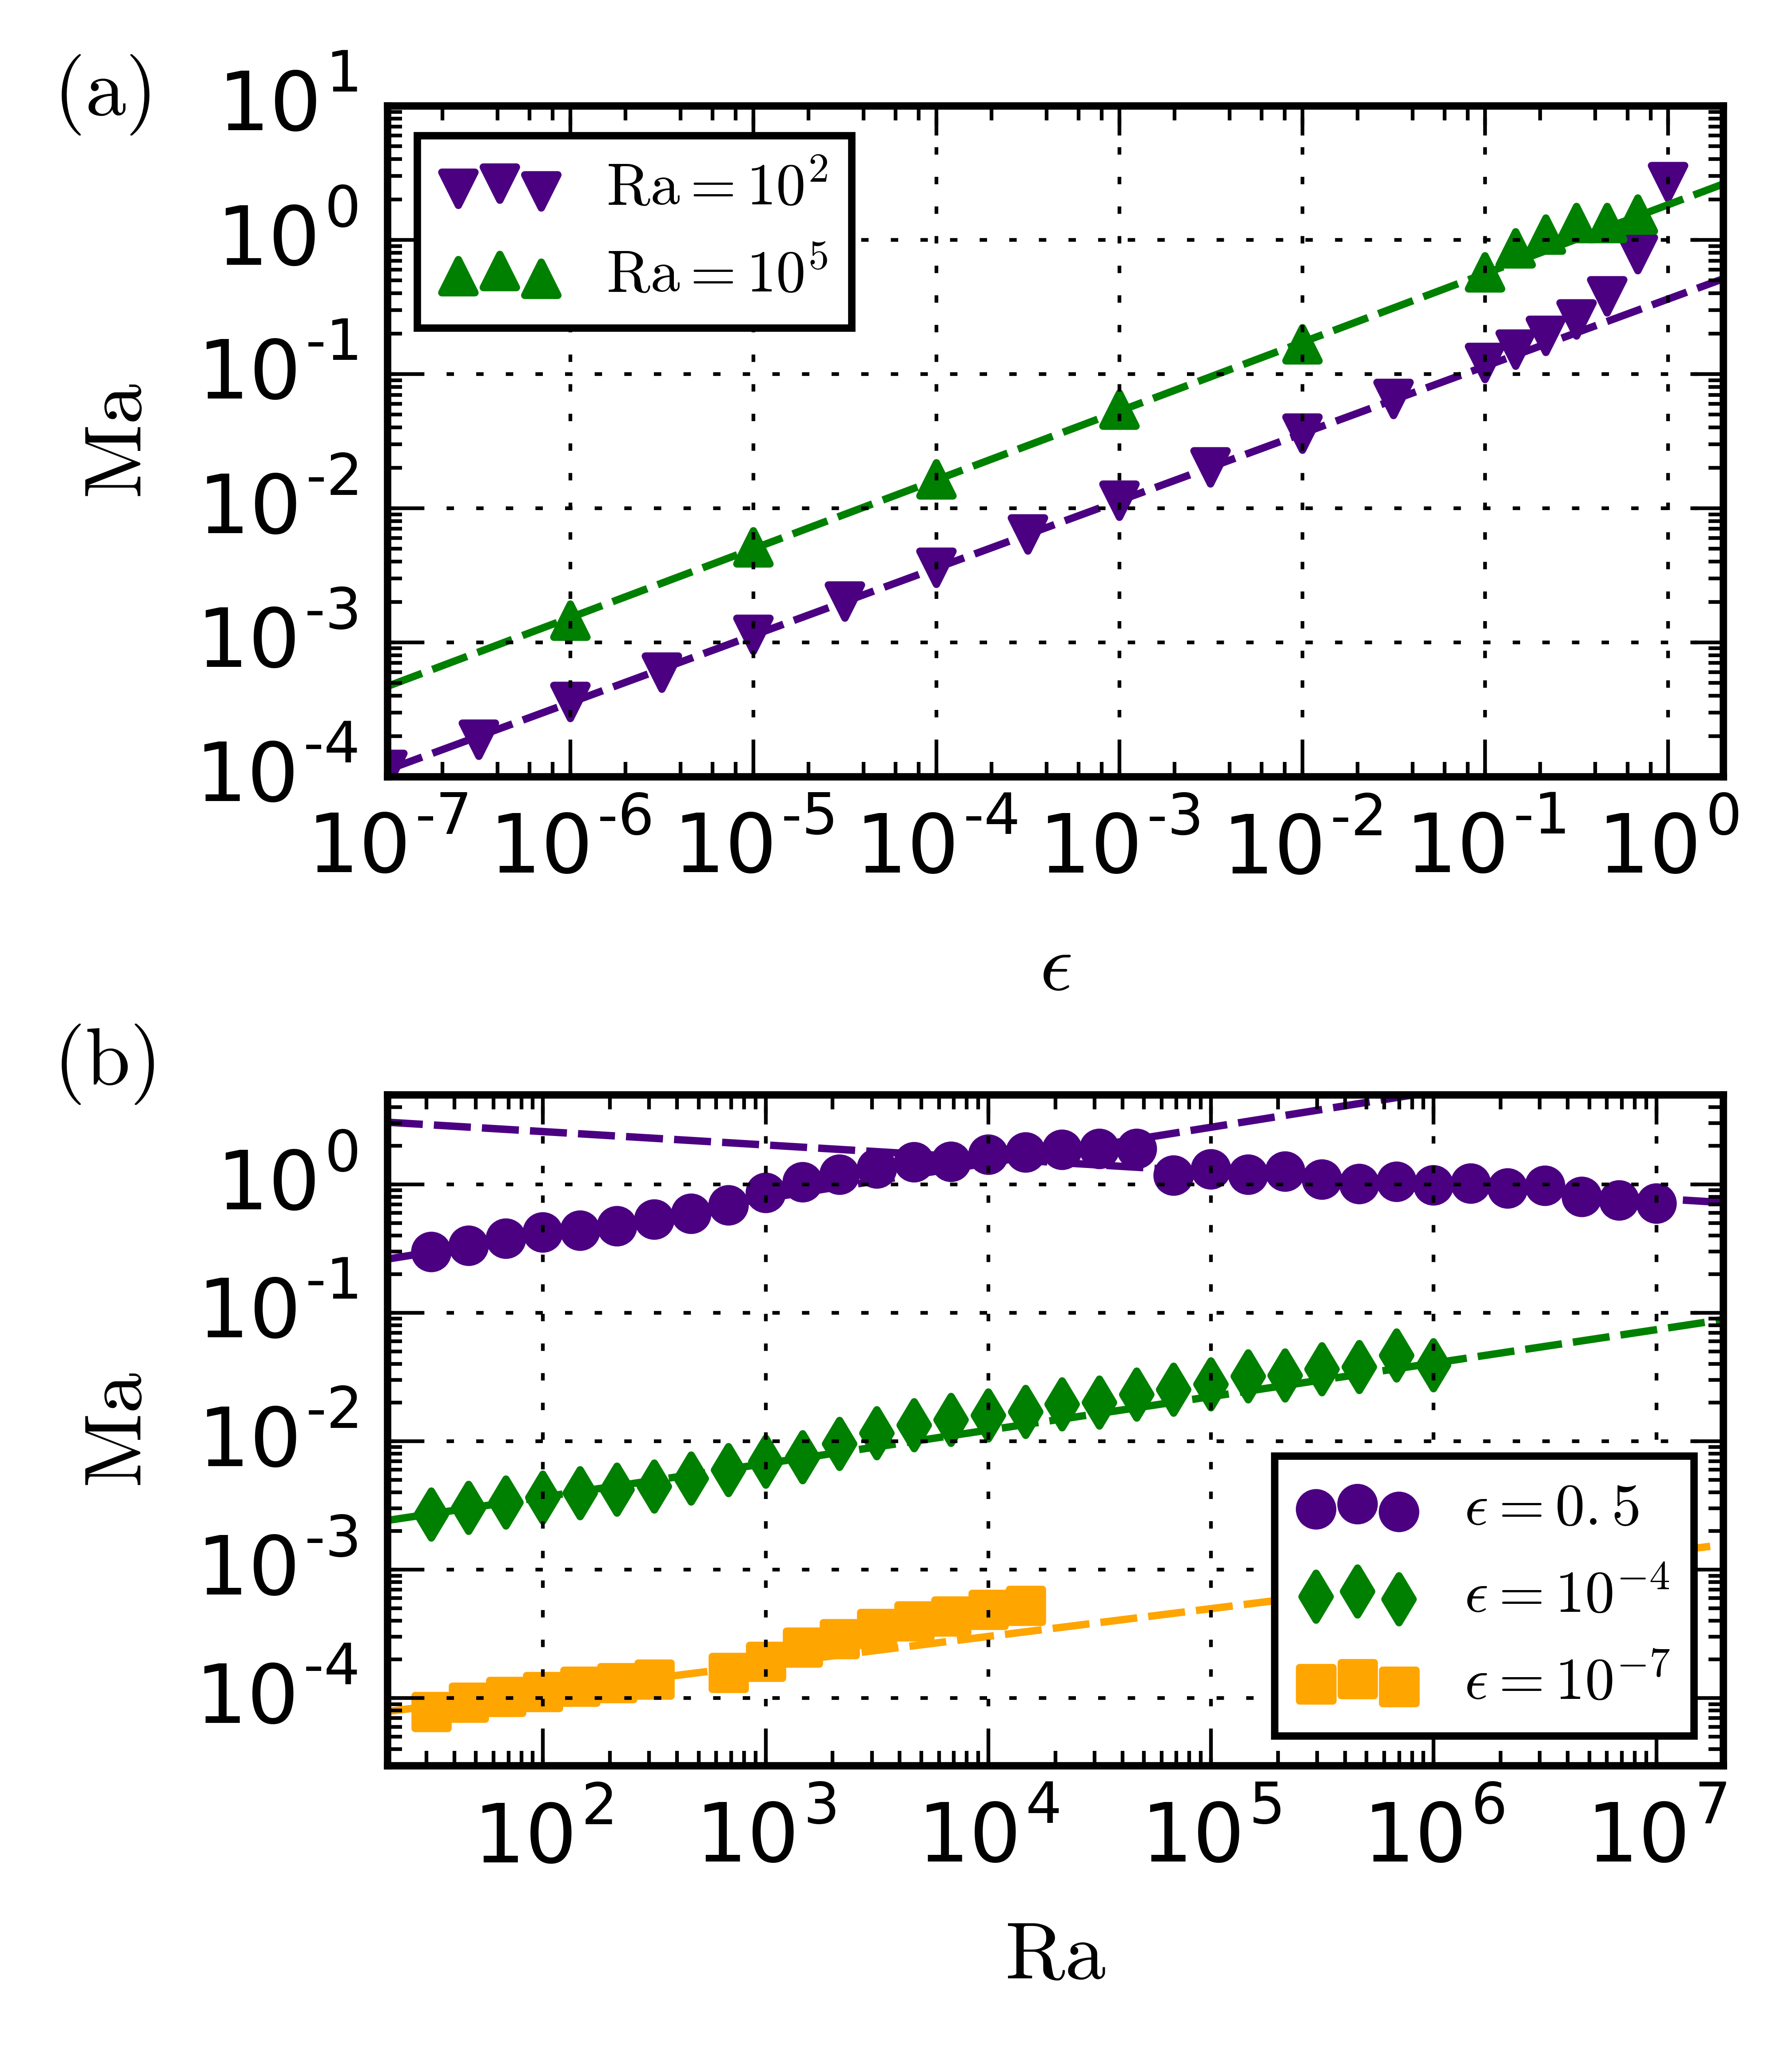
\includegraphics[width=3.4375in]{./figs/ma_v_eps.png}
\caption{Shown are characteristic mach numbers from IVPs spanning six decades of $\epsilon$, from
very low Mach number to near Mach one.  A very strong Ma $\propto \epsilon^{1/2}$ relation is clear. 
(need to actually do linear regression)
\label{fig:ma_v_eps} }
\end{figure}



We start with initial conditions of random small perturbations compared to $\epsilon$ in the temperature
field.  We evolve the Fully Compressible Navier-Stokes equations with an energy-conserving energy equation,
which take the form:
\begin{align}
&\begin{aligned}
&\frac{D \ln\rho}{D t} + \Div{\bm{u}} = 0
	\label{eqn:continuity_eqn}
\end{aligned}\\
&\begin{aligned}
&\rho\frac{D\bm{u}}{D t}=
-\grad P + \rho\bm{g} - \nabla\cdot\stressT
	\label{eqn:momentum_eqn}
\end{aligned}\\
&\begin{aligned}
\rho c_V\left(\frac{D T}{D t} + (\gamma-1)T\Div{\bm{u}}\right) + &\Div{-\kappa\grad T} = \\
&-\left(\stressT\cdot\nabla\right)\cdot\bm{u} 
	\label{eqn:energy_eqn}
\end{aligned}
\end{align}
where $D/Dt \equiv \partial_t + \bm{u}\cdot\grad$ and the viscous stress tensor is defined as
\begin{equation}
\Pi_{ij} \equiv -\mu\left(\frac{\partial u_i}{\partial x_j} + \frac{\partial u_j}{\partial x_i} - \frac{2}{3}\delta_{ij}\Div{\bm{u}}\right).
	\label{eqn:stress_tensor}
\end{equation}

In such stratified systems, the total convective flux can be defined as
\begin{equation}
\bm{F}_{\text{conv}} = \bm{F}_{\text{enth}} + \bm{F}_{\text{KE}} + \bm{F}_{\text{PE}} + \bm{F}_{\text{visc}},
\end{equation}
where $\bm{F}_{\text{enth}} \equiv \rho\bm{u}(c_V T + P/\rho)$ is the enthalpy flux, $\bm{F}_{\text{KE}} \equiv 
\rho|\bm{u}|^2\bm{u}$ is the kinetic energy flux, $\bm{F}_{\text{PE}} \equiv \rho\bm{u}\phi$ is the potential
energy flux (with $\phi \equiv -gz$), 
and $\bm{F}_{\text{visc}} \equiv \bm{u}\cdot\stressT$ is the viscous flux.  Dotting 
Eq. \ref{eqn:momentum_eqn} with $\bm{u}$ and adding it to 
Eq. \ref{eqn:energy_eqn}, we retrieve the full energy equation in conservation form,
\begin{equation}
\frac{\partial}{\partial t}\left(\rho\left[\frac{|\bm{u}|^2}{2} + c_V T + \phi\right]\right) +
\Div{\bm{F}_{\text{conv}} + \bm{F}_{\text{rad}}} = 0
	\label{eqn:energy_eqn_full}
\end{equation}
where $\bm{F}_{\text{rad}} = -\kappa \grad T$. 

The efficiency of convection is defined by the Nusselt number.  While the Nusselt number is well-defined in \RB convection
as the amount of total flux divided by the steady-state background conductive flux 
\cite{johnston&doering2009, otero&all2002},
a well-defined Nusselt number is more elusive in stratified convection.  A traditional definition of the Nusselt
number in stratified convection is \cite{graham1975,hurlburt1984}
\begin{equation}
N \equiv \frac{F_{\text{conv, z}} + F_{\text{rad, z}} - F_A}{F_{\text{ref}} - F_A},
\label{eqn:nusselt}
\end{equation}
where $F_{\text{conv, z}}$ and $F_{\text{rad, z}}$ are the z-components of $\bm{F}_{\text{conv}}$ and $\bm{F}_{\text{rad}}$,
respectively.  $F_A$ is the adiabatic conductive flux, defined as $F_A = -\kappa \grad T_{\text{ad}}$.  For an
atmosphere in hydrostatic equilibrium, such as a polytrope, $\grad T_{\text{ad}} \equiv - g / c_{P}$, and thus
$F_A = \kappa g / c_{P}$.  $F_{\text{ref}} = \Delta T / L_z$ is the conductive flux of a linear profile connecting the upper
and lower plates, where $\Delta T = T_{u} - T_{\ell}$.

Such a definition of the Nusselt number is general to both stratified and \RB convection.  Convection works to
suppress entropy stratification and create isentropic atmospheres.  Under the Boussinesq approximation where
density variations are ignored, entropy stratification is directly proportional to temperature stratification,
such that $\grad S \rightarrow 0$ only when $\grad T \rightarrow 0$.  Thus, for \RB convection, 
$\grad T_{\text{ad}} \equiv 0$ and the familiar form of $N$ is retrieved.  In the case of stratified convection,
as $\epsilon \rightarrow m_{ad} + 1$, as in \cite{brandenburg2015}, $\grad P \propto g \rightarrow 0$ and
the resulting $\grad T_{\text{ad}} \rightarrow 0$.  In such a case, $F_A \rightarrow 0$ and the familiar
definition of the \RB nusselt number is appropriate to use. However, for any given values of $\epsilon$, including
the very small values used in this work, Eq. \ref{eqn:nusselt} is the proper non-dimensional definition
of the Nusselt number.

***WE USE DEDALUS, EXPLAIN WHAT IT ARE***

***EXPLAIN BOUNDARY CONDITIONS***

***EXPLAIN WHAT THE CHARACTERISTIC TIME SCALE, THE BUOYANCY TIME, IS***


\section{Results \label{section:results}}
We ran initial value problems for a few hundreds of buoyancy times past the convective transients from 
Rayleigh numbers around $R_{crit}$ up to Rayleigh numbers of $\approx 10^7 R_{crit}$.  While bulk thermodynamic
structures are similar between low and high $\epsilon$, high $\epsilon$ runs start to exhibit shock fronts
propagating away from downflow channels, such as those in Fig. \ref{fig:entropy_snapshots}, as reported in \cite{cattaneo&all1990}.
\begin{figure}[t]
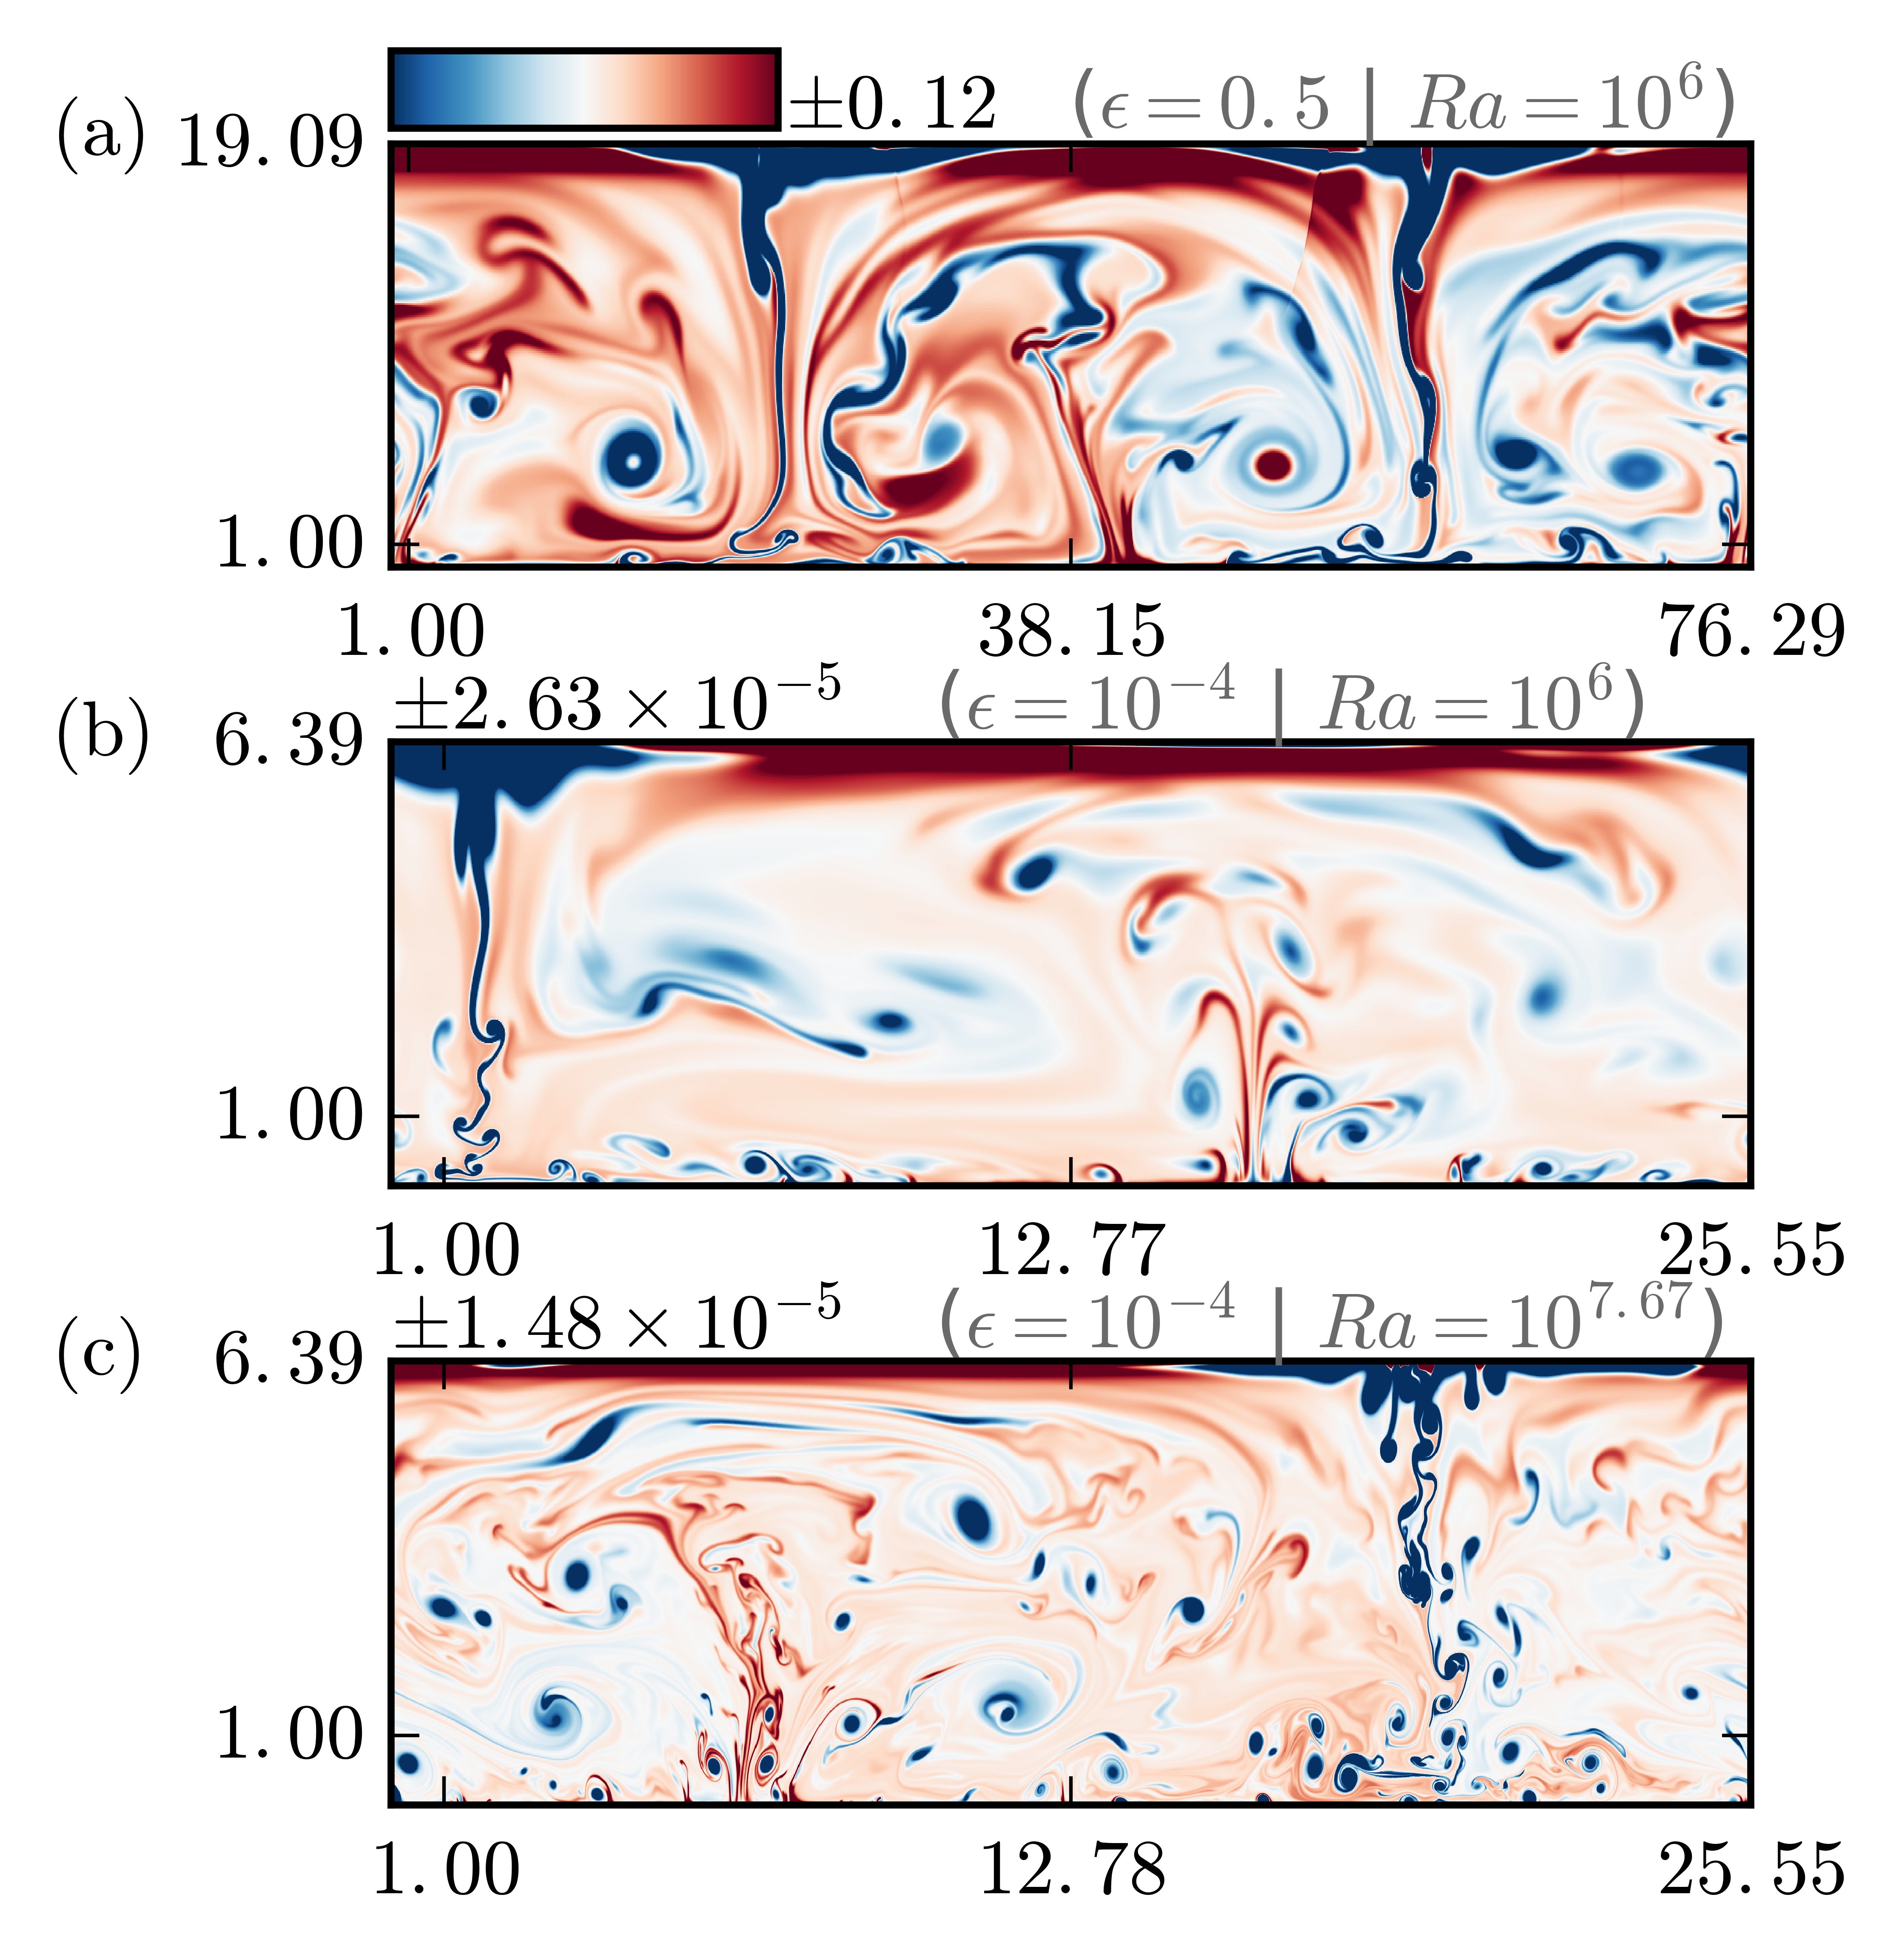
\includegraphics[width=3.4375in]{./figs/snapshots_fig.png}
\caption{Two characteristic snapshots after about 200 buoyancy times are shown at $\epsilon=10^{-4}$ (top)
and $\epsilon=0.5$ (bottom) at Ra = $10^6$.  
\label{fig:entropy_snapshots} }
\end{figure}

Despite diferent thermodynamic structures, the fluxes look fairly similar at low and high mach number (sort of?
I don't think the ones I have are averaged over enough time, especially the eps=0.5 one, but I Pleiades is
a bit slammed right now).  See Fig \ref{fig:flux_profiles}

\begin{figure}[b]
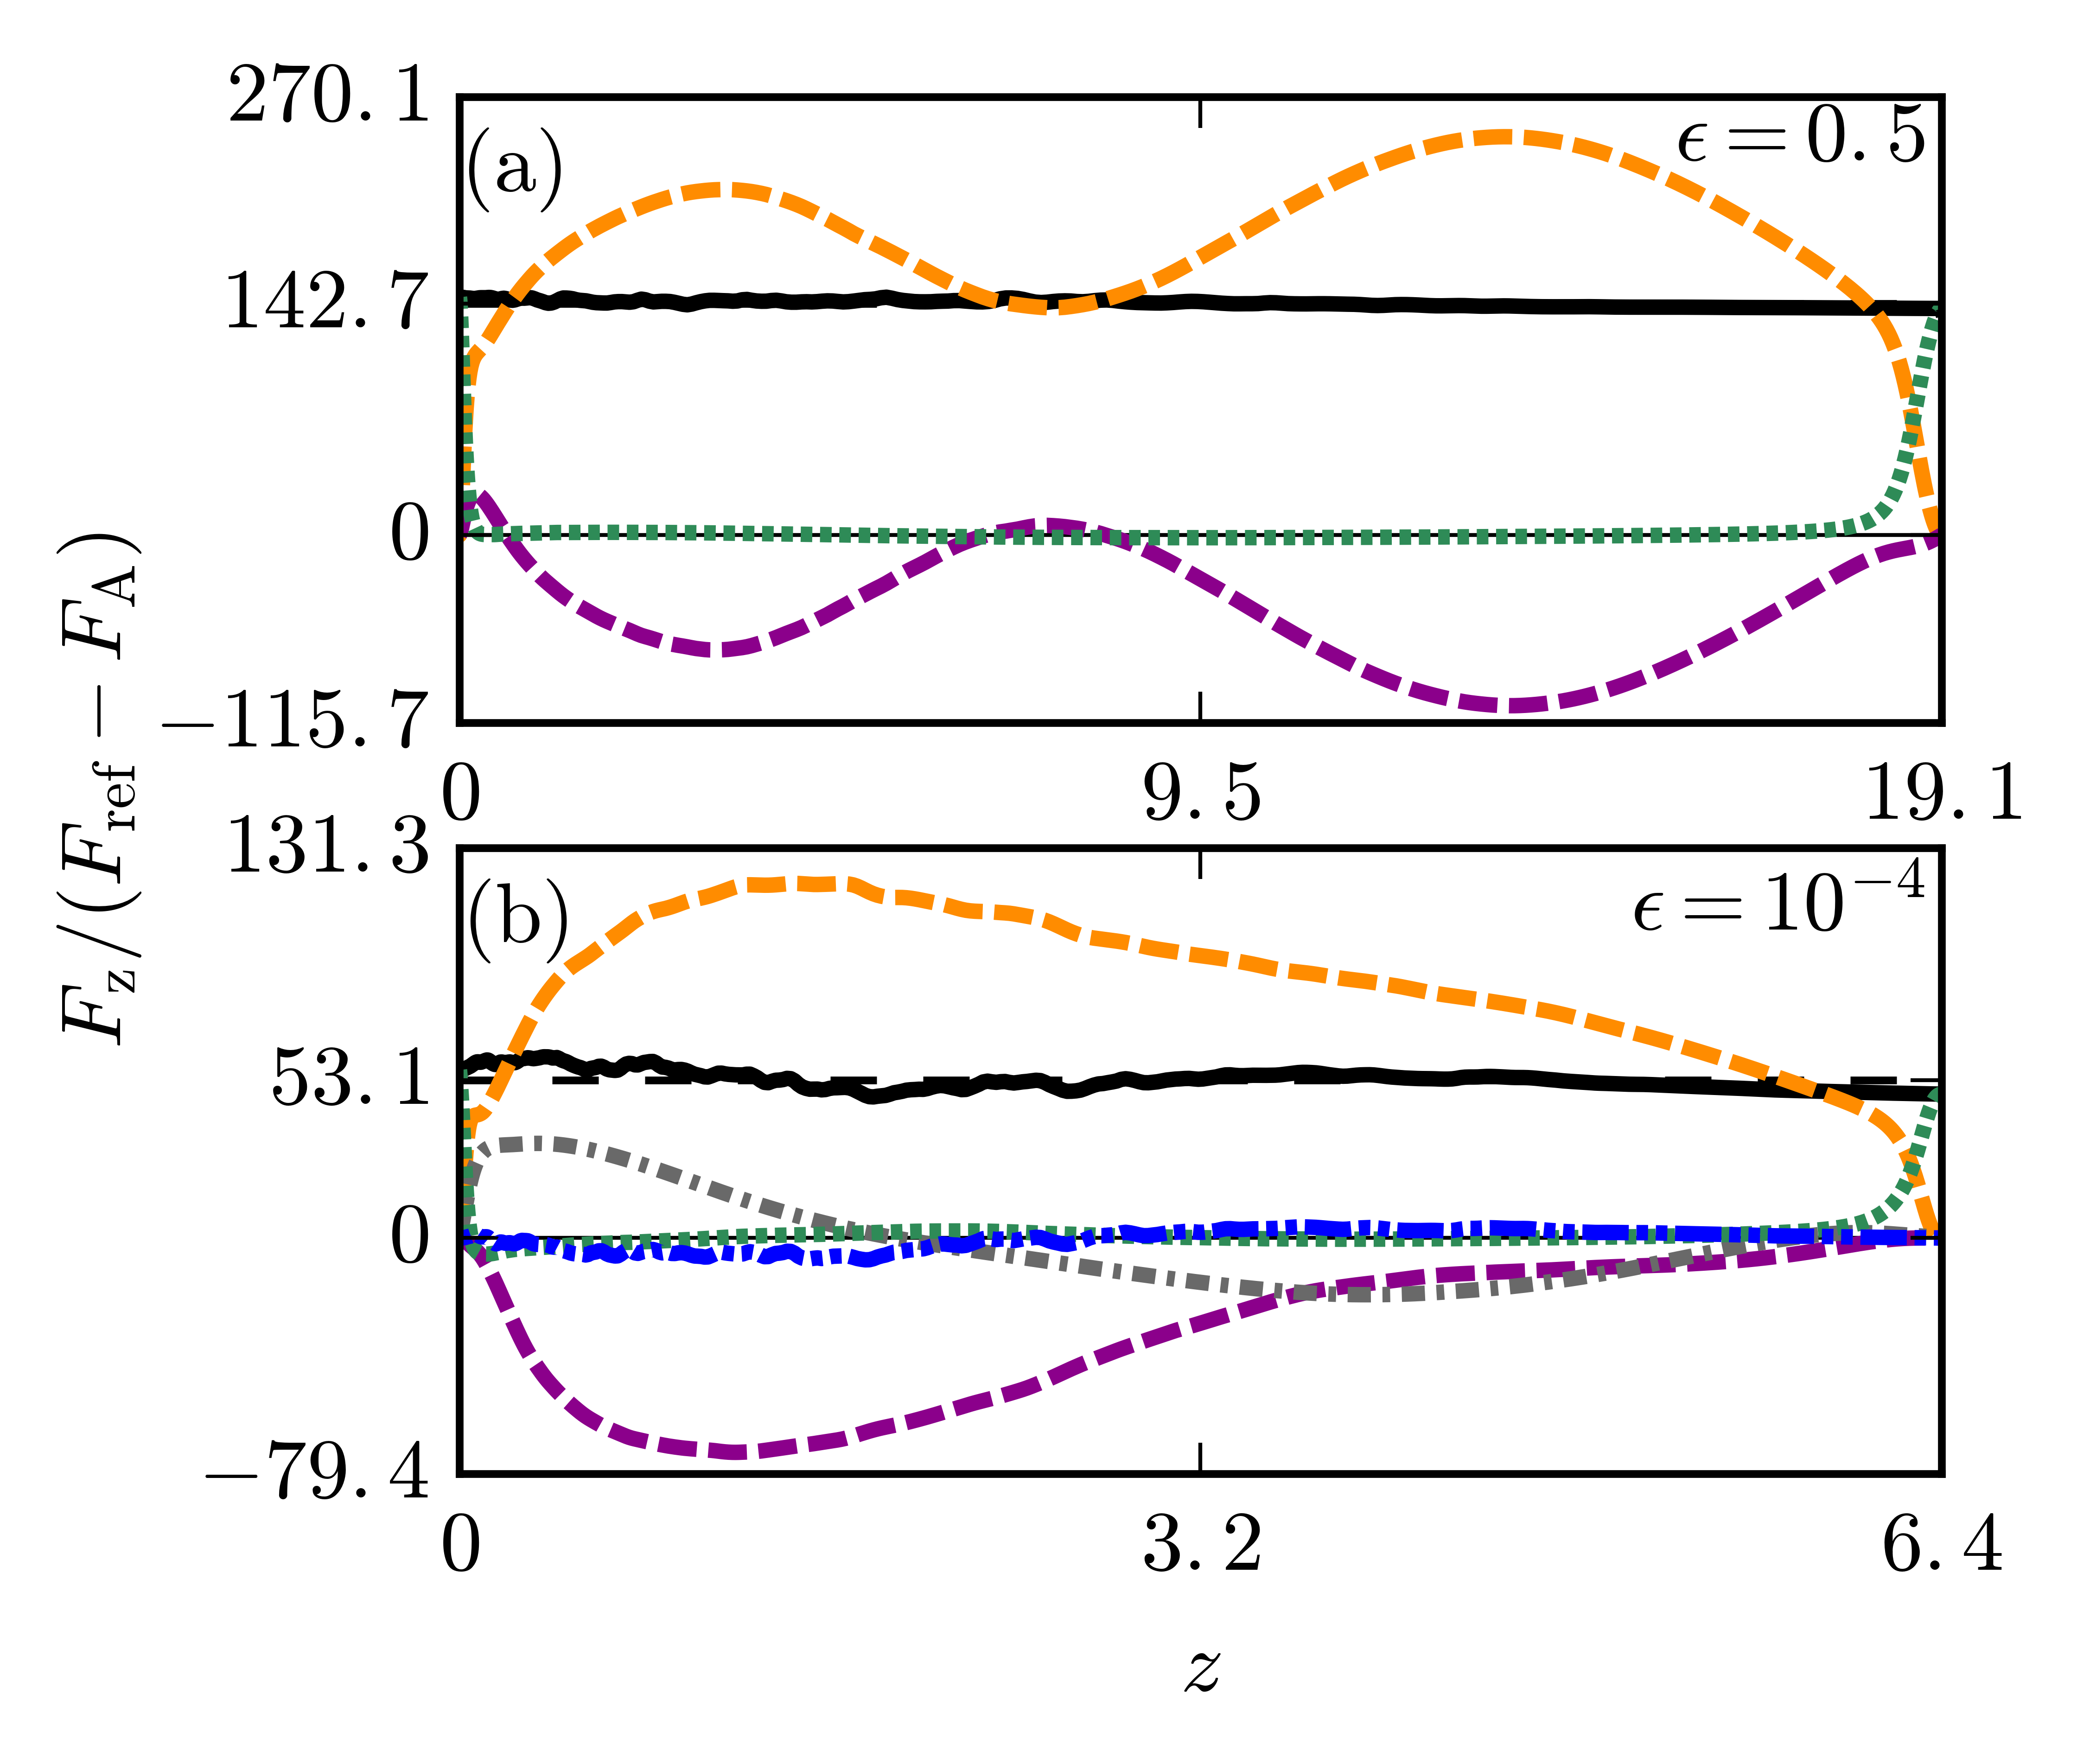
\includegraphics[width=3.4375in]{./figs/fluxes_fig.png}
\caption{Flux profiles for low (top) and high (bottom) Mach number flows.  
\label{fig:flux_profiles} }
\end{figure}

At low Rayleigh number, diffusivities are high and the flows are very laminar.  Such flows often achieve a
steady state and have a well-defined Nusselt number which is independent of time.  However, as the Rayleigh
number increases, the flows become increasingly time-dependent.  Even steady structures such as solid
``rolls'' like those pictured in Fig. \ref{fig:entropy_snapshots} have highly time-dependent Nusselt numbers.
This is, in part, due to the fact that cold downdrafts floating to the bottom of the domain can be entrained
by upflows, or warm risen parcels can be entrainedi n the intense cold downdrafts.  Such events reverse the
preferred direction of flux in the system, and even let the Nusselt number become negative for short periods of
time.  See Fig. \ref{fig:nu_v_time}.  As a result, it is necessary to take a long time average of the fluxes
before calculating the Nusselt number at higher Rayleigh number.


\begin{figure}[t]
\includegraphics[width=3.4375in]{./figs/nu_v_time.png}
\caption{The evolution of the Nusselt number is shown at low ($10^2$) and high ($10^7$) Rayleigh number and at
$\epsilon = 10^{-4}$.  At low Rayleigh number, the system is able to settle into a time invariant solution. As
the Rayleigh number is raised, the thermodynamic structure become increasingly complex and time variant, and a
time-average of the Nusselt number is required to obtain a sensible mean.
\label{fig:nu_v_time} }
\end{figure}

The evolution of the Nusselt number as the Rayleigh number is increased is shown for both high and low
$\epsilon$ in Fig. \ref{fig:nu_v_ra}.  Below convective onset, the Nusselt number is perfectly one. Just above
onset, there is a brief range of highly inflated scaling between $N$ and Ra.  From about $10R_{crit}$ to roughly
$10^{4-5}R_{crit}$, Ra and $N$ follow the relationship: (put a power law here)  Above about
$10^5 R_{crit}$, the Nusselt number flattens out as Ra is increased -- perhaps this is some Featherstone 2016
shennanigans.

\begin{figure}[b]
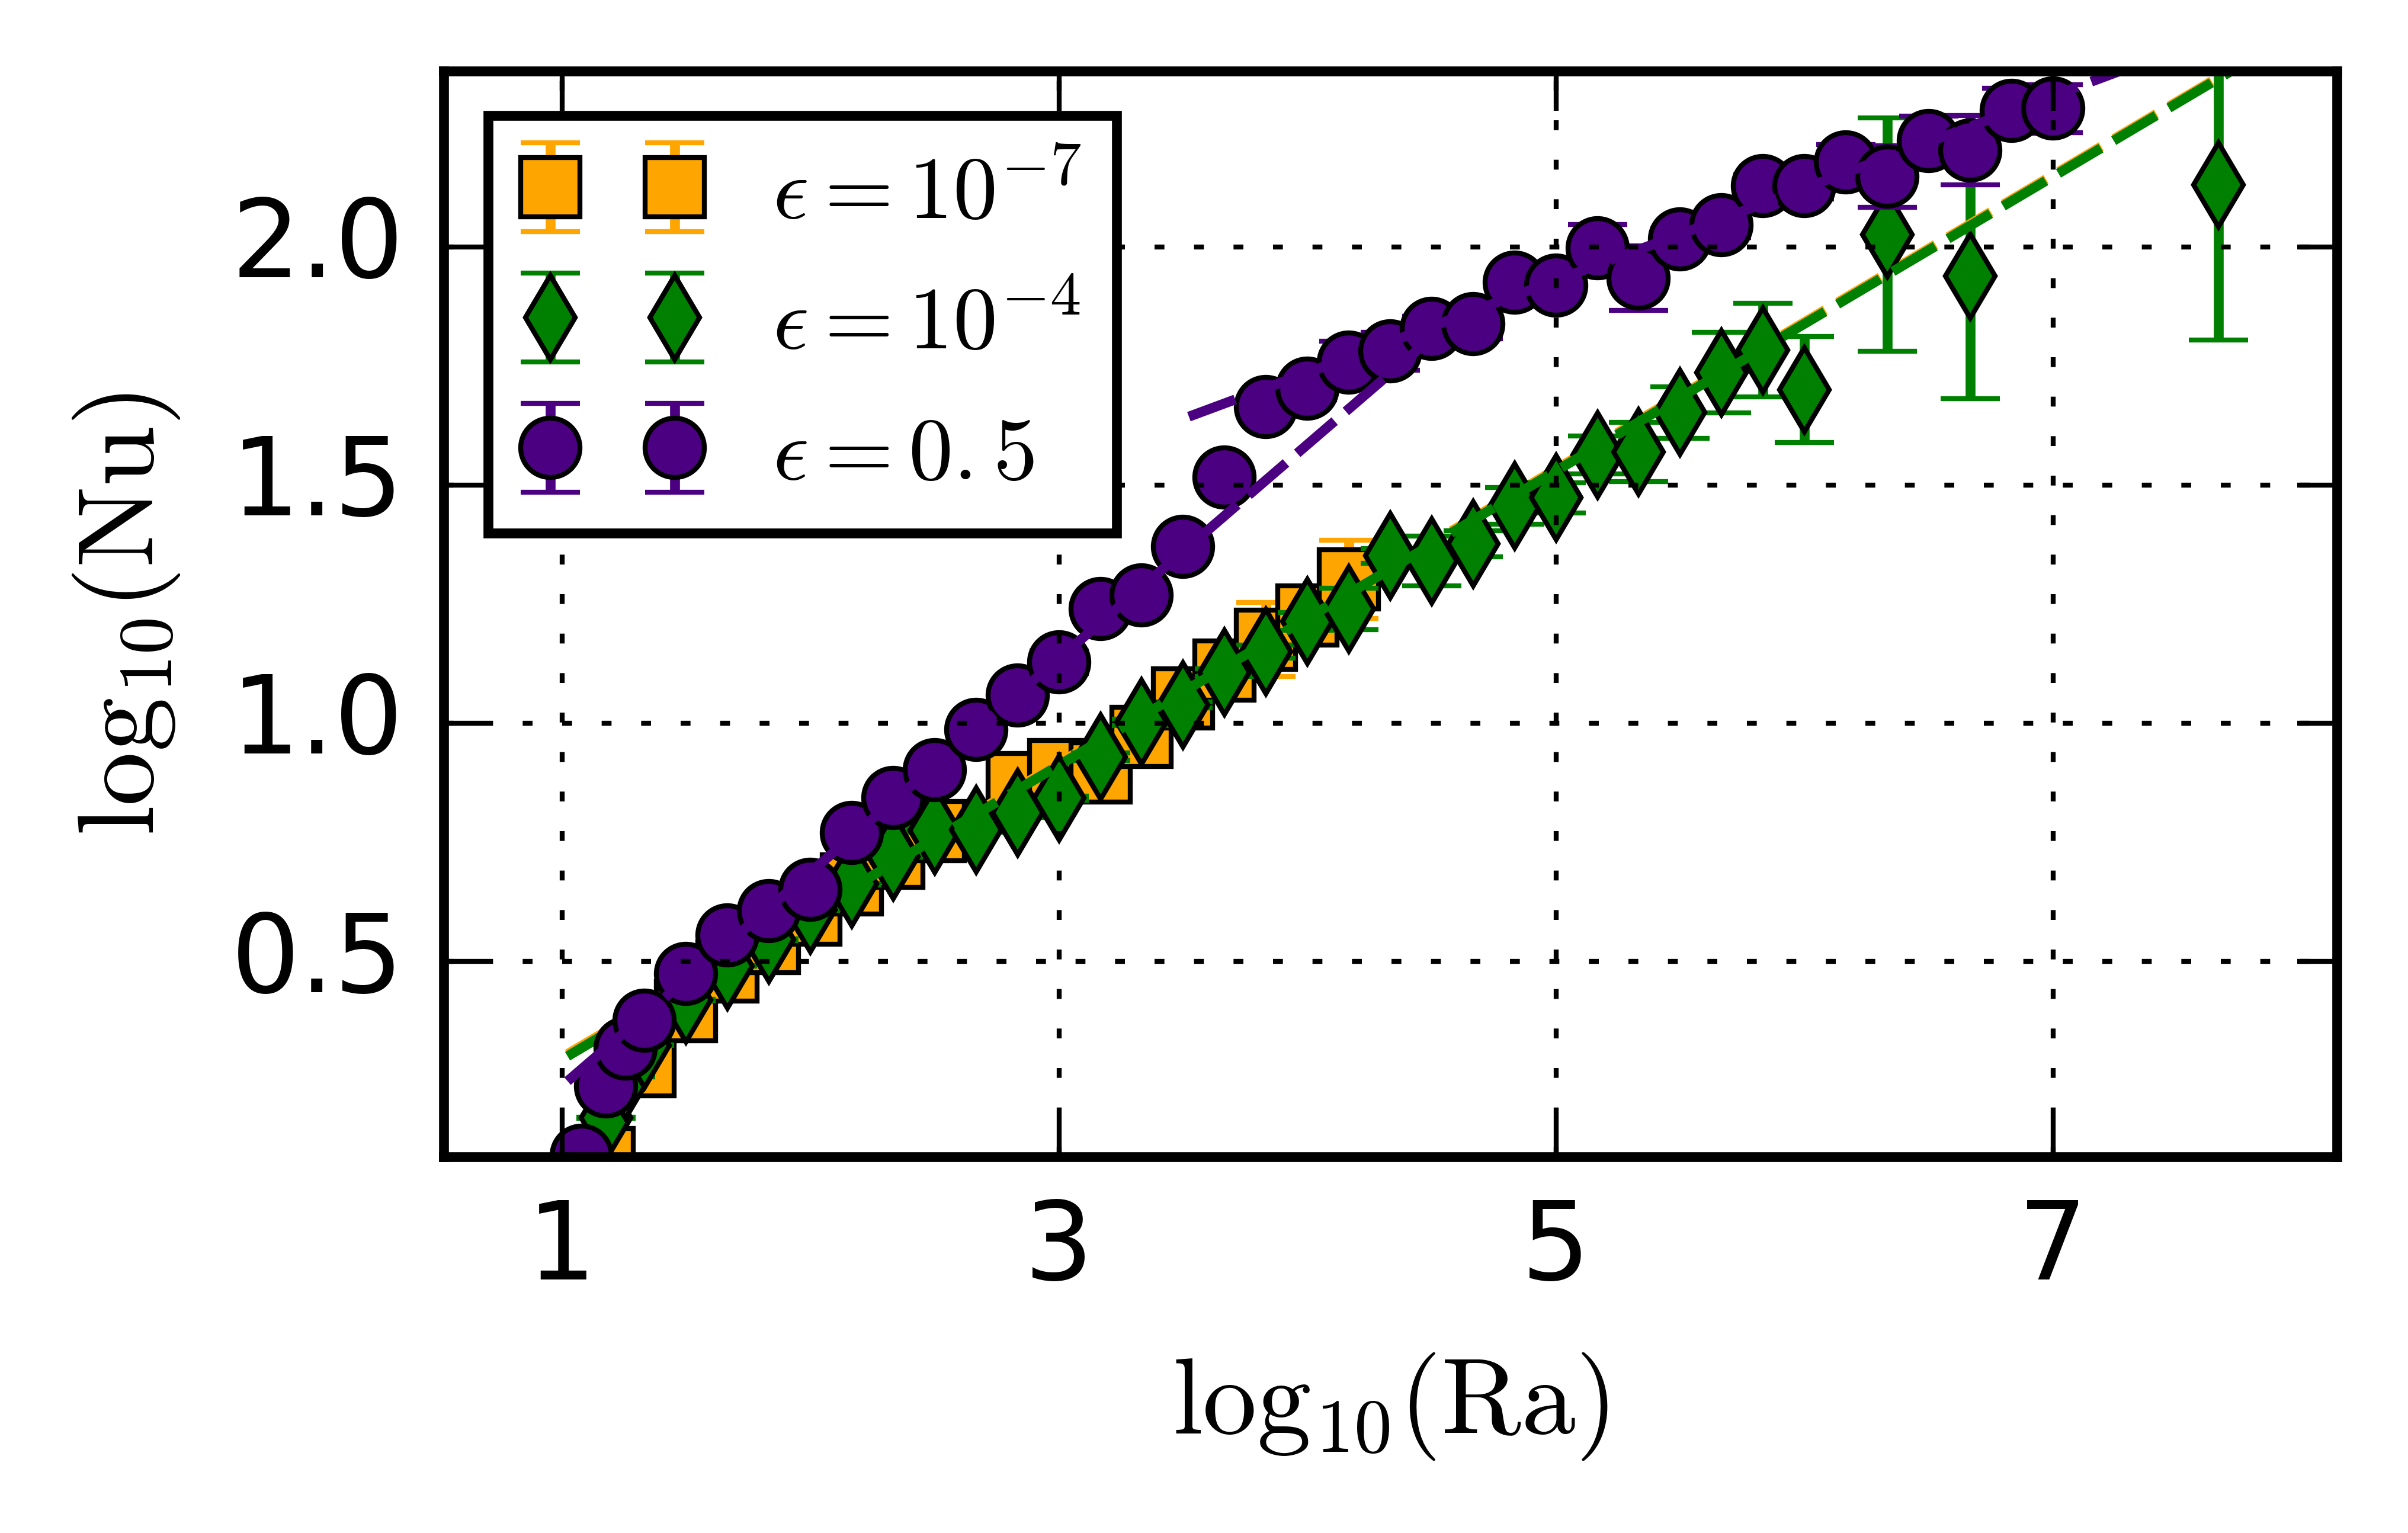
\includegraphics[width=3.4375in]{./figs/nu_v_ra.png}
\caption{Variation of the Nusselt number as a function of the Rayleigh number is shown.
\label{fig:nu_v_ra} }
\end{figure}




\begin{acknowledgements}
This work was supported by the CU/NSO Hale Graduate Fellowship and Juri's allocation and Ben's allocation.
\end{acknowledgements}

\bibliography{../biblio.bib}
\end{document}
